\documentclass{beamer}
\usetheme{Madrid}
\setbeamertemplate{footline}
{
  \leavevmode%
  \hbox{%
  \begin{beamercolorbox}[wd=.333333\paperwidth,ht=2.25ex,dp=1ex,center]{author in head/foot}%
    \usebeamerfont{author in head/foot}\insertshortauthor%~~\beamer@ifempty{\insertshortinstitute}{}{(\insertshortinstitute)}
  \end{beamercolorbox}%
  \begin{beamercolorbox}[wd=.333333\paperwidth,ht=2.25ex,dp=1ex,center]{title in head/foot}%
    \usebeamerfont{title in head/foot}\insertshorttitle
  \end{beamercolorbox}%
  \begin{beamercolorbox}[wd=.333333\paperwidth,ht=2.25ex,dp=1ex,right]{date in head/foot}%
    \usebeamerfont{date in head/foot}\insertshortdate{}\hspace*{2em}
    \insertframenumber{} / \inserttotalframenumber\hspace*{2ex} 
  \end{beamercolorbox}}%
  \vskip0pt%
}
\usepackage[utf8]{inputenc}
\usepackage[T1]{fontenc}
\usepackage[francais]{babel}
\usepackage{graphicx}
\usepackage{verbatim}
\title{La description de données avec XML}
\author{Julien Lemattre\and Axel Veber}
\institute{julien.lemattre@etud.univ-montp2.fr \and axel.veber@etud.univ-monpt2.fr}
\AtBeginSection[]
{
  \begin{frame}<beamer>{Table des matières}
    \tableofcontents[currentsection]
  \end{frame}
}
%------------------------------ Document ---------------------------------

\begin{document}

\begin{frame}
  \titlepage
\end{frame}

\begin{frame}{Table des matières}
  \tableofcontents
  % You might wish to add the option [pausesections]
\end{frame}

%------------------------------------------Contenu----------------------------------------------

\section{Histoire de XML} %1ere partie-------------------------------------

\begin{frame}{Histoire de XML}{Origine du XML}
  \begin{itemize}
  \item {
    Problêmatique : communication par Internet avec des fichiers.
  }
  \item {
    Chaque programmes avaient leurs façons de gérer les fichiers.
  }
  \item{
    SGML (\textbf{S}tandard \textbf{G}eneralized \textbf{M}arkup \textbf{L}anguage) a été crée pour standardiser la gestion de fichier.
  }
  \item{
    Cependant, SGML était trop complexe pour permettre la communication entre machines.
  }
  \end{itemize}
\end{frame}

\begin{frame}{Histoire de XML}{Apparition de XML 1.0 et 1.1}
    \begin{itemize}
    \item {
        XML (e\textbf{X}tensible \textbf{M}arkup \textbf{L}anguage)est né du compromis entre SGML et la communication sur le Web.
    }
    \item{
        XML 1.0 est devenu une recommandation du W3C le 10 février 1998.
    }
    \item{
        XML 1.1 a été publié le 4 février 2004 en ajoutant le support de caractères Unicode 2.0.
    }
    \item{
        Cependant, XML 1.0 reste la version la plus utilisée.
    }
    \end{itemize}
\end{frame}{}{}

\section{Principes de XML} %2eme partie ------------------------------------

\begin{frame}{Principes de XML}{Ce que XML permet}
    \begin{itemize}
    \item{
        XML facilite l'échange entre les machines sur Internet entre programmes car c'est un langage standardisé
    }
    \item{
        C'est un langage qui est comprit autant par les machines que pour l'être humain car il est lisible et permet de donner des noms aux données
    }
    \end{itemize}
    \begin{alertblock}{Remarque}
        XML n'est pas un langage de programmation : ce langage décrit des données sans les exploiter.
    \end{alertblock}
\end{frame}

\begin{frame}{Principes de XML}{Structure d'un fichier XML}
        Les données décrites par un fichier XML sont organisées sous forme d'arborescence\\
        \begin{figure}
        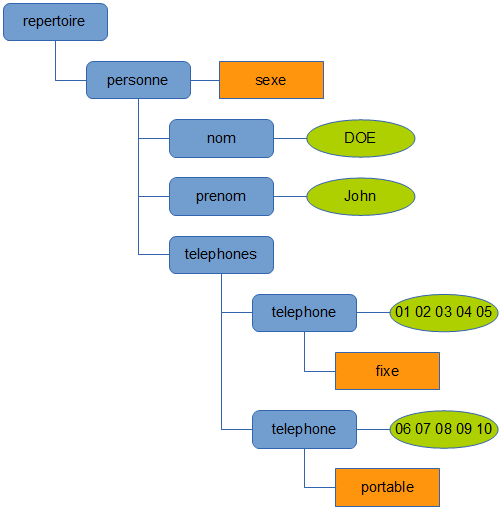
\includegraphics[scale=0.35]{421530.png}
        \caption{Structure d'une personne dans un répertoire}
        \end{figure}
\end{frame}

\section{Syntaxe de XML}%3eme partie --------------------

\subsection{Langage de balises}


\begin{frame}{Syntaxe de XML}{Langage de balises}

Deux types de balises : simples et doubles.
\begin{exampleblock}{Exemple}
\alert{\textless balise\textgreater}Contenu de la balise\alert{\textless/balise\textgreater} : exemple de balise double\\
\alert{\textless balise/\textgreater} : exemple de balise simple
\end{exampleblock}

\begin{alertblock}{Attention}
Les balises ouvrantes et fermantes doivent avoir \alert{exactement} le même nom.
\end{alertblock}

\end{frame}


\begin{frame}{Syntaxe de XML}{Langage de balises}
\begin{itemize}
\item Une balise simple est une balise double qui n'a pas de contenu. C'est un raccourci.\\
\item{Une balise double peut tout contenir : chaîne, entiers, autres balises...}
\item{Attention cependant à ne pas croiser les balises, mais à les encapsuler.}

\end{itemize}
\end{frame}

\begin{frame}{Syntaxe de XML}{Langage de balises}
La généricité du XML vient de la possibilité de créer son propre langage balisé. Cependant, 
des conventions de nommage des balises doivent être respectées : 
\begin{itemize}
\item Les noms peuvent contenir chiffres, lettres et carctères spéciaux.
\item{Mais ils ne peuvent pas débuter par un chiffre ou un caractère de ponctuation.}
\item{Ils ne peuvent pas non plus commencer par la chaîne "XML".}
\item{Ils ne contiennent ni espaces, ni les caractères suivants : - , ; , \textless et \textgreater .}
\end{itemize}
\end{frame}

\begin{frame}{Syntaxe de XML}{Langage de balises}
Deux parties distinctes : le prologue et le corps.
\begin{itemize}
\item Le prologue :
\begin{exampleblock}{Exemple de prologue}\textless?xml version = "1.0" encoding="UTF-8" standalone="yes" ?\textgreater
\end{exampleblock}
\item Le corps : 
\begin{exampleblock}{Exemple de corps}
  \textless racine\textgreater\\
  \textless balise\_paire\textgreater texte\textless/balise\_paire\textgreater\\
  \textless balise\_paire2\textgreater texte\textless/balise\_paire2\textgreater\\
  \textless balise\_paire\textgreater texte\textless/balise\_paire\textgreater\\
\textless/racine\textgreater
\end{exampleblock}

\end{itemize}
\end{frame}

\begin{frame}{Syntaxe de XML}{Langage de balises}
\begin{itemize}
\item 3 informations dans le prologue :
    \begin{itemize}
    \item La version de XML
    \item L'endodage utilisé
    \item L'autosuffisance du document
    \end{itemize}
\item Dans le corps, il doit y avoir une paire de balises qui contient toutes les autres.\\
On l'appelle racine.
\end{itemize}

\end{frame}

\subsection{Attributs}
\begin{frame}{Syntaxe du XML}{Attributs}
On peut ajouter des informations supplémentaires aux balises : les attributs.\\
Le nom est au choix.
\begin{exampleblock}{Exemple d'attribut}
    \begin{verbatim}
        \textless prix devise="euro"\textgreater25.3\textless/prix\textgreater
    \end{verbatim}
\end{exampleblock}
L'information principale est le montant du prix, mais la devise est une\\
information supplémentaire qui caractérise le prix.
\end{frame}

\begin{frame}{Syntaxe du XML}{Attributs}
Il peut y avoir ou non plusieurs attributs.\\
Quelques règles :
\begin{itemize}
\item Même règle de nommage que pour les balises
\item La valeur de l'attribut doit être entre guillemets
\item Pas de doublons à l'intéreur d'une balise.
\end{itemize}
\end{frame}

\subsection{Document bien formé}
\begin{frame}{Syntaxe du XML}{Document bien formé}
Quqlques règles définissent si un document est "bien formé", ou "well-formed" :
\begin{itemize}
\item Si XML 1.1, le prologue doit être complet
\item Une seule racine
\item Noms des balises et attributs conformes
\item Valeurs des attributs entre guillemets
\item Aucun chevauchement de balises
\end{itemize}

Si ces règles ne sont pas respectées, le document est inutilisable.
\end{frame}

\section{Descriptions de documents XML}%4eme partie --------------------------------

\subsection{Pourquoi définir ses données}
\begin{frame}{Descriptions de documents XML}{Pourquoi définir ses données}
    \begin{itemize}
    \item{
        Maintenant qu'un document est dit "bien formé", il faut l'exploiter.
    }
    \item{
        Afin d'être régulier dans l'exploitation d'un fichier XML, il faut qu'il soit \textbf{valide}.
    }
    \item{
        Un document \textbf{valide} obéit à une définition des données qu'il décrit.
    }
    \item{
        Ainsi, plusieurs concepteurs peuvent se mettre d'accord sur une grammaire commune.
    }
    \item{
        Pour décrire un document, plusieurs formats sont possibles. Ici, on parlera de DTD (Document Type Definition)
    }
    \item{
        Cette définition pourra être écrit dans le document XML, où dans un autre fichier (ici, on parlera de fichier .dtd).
    }
    \end{itemize}
\end{frame}

\subsection{Définir la structure}
\begin{frame}{Descriptions de documents XML}{Définir la structure}
    On définit le "squelette" de notre arborescence en définissant les balises avec cette syntaxe :
    \begin{verbatim}
        <!ELEMENT balise (contenu)>
    \end{verbatim}
    \begin{itemize}
    \item{
        On indique la balise qu'on définit.
    }
    \item{
        On indique ce qu'elle doit contenir.
    }
    \end{itemize}
\end{frame}

\begin{frame}{Descriptions de documents XML}{Définir la structure}
    Le contenu d'une balise peut être défini comme suit :
    \begin{description}
    \item[\#PCDATA]{
        Indique qu'une balise peut contenir une chaîne de caractère, un entier...
    }
    \item[balise]{
        Indique qu'une balise doit \textbf{obligatoirement} contenir la balise indiquée.
    }
    \item[balise?]{
        Indique que la balise \textbf{peut} contenir la balise indiquée
    }
    \item[b1, b2]{
        Indique qu'une balise doit \textbf{obligatoirement} contenir les balises indiquées \textbf{dans cet ordre}.
    }
    \item[b1 | b2]{
        Indique que la balise doit \textbf{obligatoirement} contenir une des balises indiquées \textbf{dans cet ordre}.
    }
    \end{description}
\end{frame}

\begin{frame}{Descriptions de documents XML}{Définir la structure}
    \begin{description}
        \item[balise*]{
            Indique que la balise peut être \textbf{répetée}, même si elle est \textbf{optionnelle}.
        }
        \item[balise+]{
            Indique que la balise peut être \textbf{répetée}.
        }
    \end{description}
    \begin{exampleblock}{Exemple}
    \begin{verbatim}
        <!ELEMENT repertoire (personne+)>\\
        <!ELEMENT personne (nom, prenom, adresse, telephone?)>\\
        <!ELEMENT nom (\#PCDATA)>\\
        <!ELEMENT prenom (\#PCDATA)>\\
        <!ELEMENT adresse (\#PCDATA)>\\
        <!ELEMENT telephone (\#PCDATA)>
    \end{verbatim}
\end{exampleblock}
\end{frame}

\subsection{Définir les attributs}
\begin{frame}{Descriptions de documents XML}{Définir les attributs}
    Une fois l'arborescence défini, il faut définir les attributs possibles de chaque balises avec la ligne :
    \begin{verbatim}
        <!ATTLIST balise attribut type mode>
    \end{verbatim}
    \begin{description}
        \item[balise]{Le nom de la balise dans laquelle on définit l'attribut.}
        \item[attribut]{Le nom de l'attribut que la balise peut avoir.}
        \item[type]{Le type de valeur que peut prendre l'attribut : du texte non parsé (CDATA), un choix (valeur1 | valeur2) ou un identifiant.}
        \item[mode]{Indique si l'attribut doit être renseigné (\#REQUIRED), optionnel (\#IMPLIED), une constante (\#FIXED "valeur") ou une valeur par défaut.}
    \end{description}
\end{frame}

\begin{frame}{Descriptions de documents XML}{Définir les attributs - Indentifiants}
    Il est possible de donner à un n\oe ud un attribut qui lui sert d'identifiant unique. Il suffit donc de renseigner le type de l'attribut dans notre définition : 
    \begin{description}
        \item[ID]{L'attribut défini est un identifiant. Le document ne sera pas valide si un autre n\oe ud à le même identifiant.}
        \item[IDREF]{L'attribut défini se référe à un identifiant. Si l'identifiant indiqué n'existe pas, le document ne sera pas valide.}
    \end{description}
    \begin{exampleblock}{Exemple}
        \begin{verbatim}
            <!ATTLIST father id ID \#REQUIRED>\\
            <!ATTLIST child id ID \#IMPLIED>\\
            <!ATTLISE child father IDREF \#REQUIRED>\\
        \end{verbatim}
    \end{exampleblock}
\end{frame}

\section{Exemple d'API}%5eme partie -----------------------------------------------

\subsection{L'API DOM}
\begin{frame}{Exemple d'API}{L'API DOM}
    \begin{itemize}
    \item{
        Les applications utilisent des parseurs XML afin d'extraire les informations d'un document (noeuds, attributs, contenus, commentaires...).
    }
    \item{
        Ici, on parlera de DOM (\textbf{D}ocument \textbf{O}bject \textbf{M}odel).
    }
    \item{
        DOM est un standard W3C depuis 1998.
    }
    \item{
        Il est implémenté dans divers langages de programmation (C, C++, Java, PHP...). Ici, nous verrons comment utiliser le parseur en Java.
    }
    \item{
        Il est également possible pour DOM de vérifier si un document est valide selon son fichier .dtd .
    }
    \end{itemize}
\end{frame}

\subsection{Extraction de contenu en Java}
\begin{frame}{Exemple d'API}{Extraction de contenu en Java}
    Afin d'extraire les informations avec le parseur, plusieurs classes sont utilisées afin de représenter les informations du document XML :
    \begin{description}
        \item[Document]{Se référe au document XML à parser.}
        \item[Node]{C'est un élement du document XML. Il peut être un n\oe ud, un attribut ou le contenu d'une balise.}
        \item[NodeList]{Une liste de Node.}
        \item[Element]{Représente une balise du document XML. La classe Element possède d'autres fonctionnalités, comme récupérer un attribut correspondant.}
        \item[Attr]{Représente un attribut d'une balise (nom + valeur).}
        \item[Text]{Représente le contenu d'une balise.}
    \end{description}
\end{frame}

\begin{frame}{Exemple d'API}{Extraction de contenu en Java - Méthode}
    \begin{itemize}
    \item{
        On commence à créer une instance de DocumentBuilderFactory.
    }
    \item{
        L'instance de DocumentBuilderFactory permet de créer un DocumentBuilder.
    }
    \item{
        Le DocumentBuilder permet de créer un Document (à partir de là, on spécifie le document XML qu'on veut parser).
    }
    \item{
        On extrait l'élement racine dans un Element grâce au Document.
    }
    \item{
        Selon la structure de l'arborescence du document, on récupère la liste des n\oe uds fils dans un NodeList.
    }
    \item{
        Dès qu'une donnée doit être présente (attribut ou contenu texte), on récupère le n\oe ud correspondant dans un Element, qui va nous permettre d'accéder aux données souhaitées.
    }
    \end{itemize}
\end{frame}

\section{Synthèse}%6eme partie-------------------------------------------------------
\begin{frame}{Synthèse}
    \begin{itemize}
    \item{
        XML est un langage de \textbf{description de données} standardisé, qui est orienté vers l'échange de données sur Internet.
    }
    \item{
        Le langage utilise des \textbf{balises}, caractérisées par des \textbf{attributs}, qui peuvent contenir d'autres balises sous forme d'\textbf{arborescence}, ou du \textbf{texte}.
    }
    \item{
        Un document \textbf{bien formé} respecte la syntaxe XML, tandis qu'un document \textbf{valide} respecte la définition proposée.
    }
    \item{
        Un document valide permet de mettre d'accord plusieurs concepteurs sur une grammaire commune, et impose une certaine rigueur lors de la création de documents XML.
    }
    \item{
        On exploite un document XML avec un \textbf{parseur XML}, qui parcours l'arborescence du document afin d'en extraire le contenu.
    }
    \end{itemize}
\end{frame}

\end{document}


